\documentclass[10pt]{ctexart}
\usepackage[a4paper,margin=22mm]{geometry}
\usepackage{amsmath,amssymb,mathtools}
\usepackage{stmaryrd}
\usepackage{booktabs,array}
\usepackage{tikz}
\usepackage{float}
\usepackage[hidelinks]{hyperref}

\newcommand{\FV}{\mathsf{FV}}
\newcommand{\Fib}{\mathsf{Fiber}}
\newcommand{\Store}{\mathsf{Store}}
\newcommand{\Bool}{\mathsf{Bool}}
\newcommand{\false}{\mathsf{false}}
\newcommand{\true}{\mathsf{true}}
\newcommand{\restr}{\mathord{\upharpoonright}}
\newcommand{\fiber}[2]{#1\mathbin{\triangleright}#2}
\newcommand{\rfcomp}{\mathbin{\blacktriangleright}}
\newcommand{\modelsr}{\mathrel{\models}}

\title{Fiber-Guided Support Refinement and Type Negation}
\author{}
\date{}

\begin{document}
\pagestyle{plain}
\maketitle

\section{Support padding}

A qualifier is represented by a declared finite support and a predicate over
stores on exactly that support:
\[
  \phi=(D_\phi,\llbracket\phi\rrbracket),
  \qquad D_\phi=\FV(\phi).
\]
For a finite set $X$, define support padding $X.\{\phi\}$ by
\[
  \FV(X.\{\phi\})=X\cup\FV(\phi),
  \qquad
  \sigma\modelsr X.\{\phi\}
  \;\Longleftrightarrow\;
  (\sigma\restr_{\FV(\phi)})\modelsr\phi.
\]
Padding changes what is observed, not the predicate after projection.  In
particular, $\{x\}.\{\top\}$ is true on every store over $x$, but unlike an
empty-support top it explicitly observes $x$.

Expected equations include
\[
  \varnothing.\{\phi\}\equiv\phi,
  \qquad
  X.\{Y.\{\phi\}\}\equiv(X\cup Y).\{\phi\},
  \qquad
  X\subseteq\FV(\phi)\Rightarrow X.\{\phi\}\equiv\phi.
\]
Here equivalence includes agreement of declared support, not merely
pointwise logical equivalence.

\section{The right-facing fiber operator}

For a finite set $X$, the formula $\fiber{X}{P}$ is interpreted by fixing the
values of $X$ and checking the substituted formula in each corresponding
fiber:
\begin{equation}\label{eq:fiber}
  r\modelsr\fiber{X}{P}
  \quad\Longleftrightarrow\quad
  \forall \sigma_X\in r\restr_X.\;
  \Fib(r,X,\sigma_X)\modelsr\sigma_X(P).
\end{equation}
This is the paper-level form of the artifact's \texttt{FFibVars} connective.

At formula level, write the right-facing fiber composition as
\begin{equation}\label{eq:fcomp}
  P\rfcomp Q
  \;\triangleq\;
  P\land\fiber{\FV(P)}{Q}.
\end{equation}
The order matters: $Q$ may depend on choices exposed by $P$.

\section{Relationship with separating conjunction}

Under the artifact's Cartesian resource product, separating conjunction
entails both orders of fiber composition:
\begin{equation}\label{eq:star-to-fiber}
  P*Q\modelsr P\rfcomp Q,
  \qquad
  P*Q\modelsr Q\rfcomp P.
\end{equation}
The product contains every compatible combination of a $P$-store and a
$Q$-store.  Fixing either support therefore preserves all choices supplied by
the other operand.

There is an exact fragment in which both implications reverse.  Let
\[
  P\triangleq x:[b_1\mid\phi],
  \qquad
  Q\triangleq y:[b_2\mid\psi],
  \qquad x\neq y,
\]
where both formulas are atomic Under bindings, their supports are disjoint,
and both typed qualifiers are inhabited.  Define their canonical covered
value sets $A$ and $B$.  Under requires every point in $A$ and $B$ to be
covered.  Hence either directional fiber composition contains the complete
rectangle $A\times B$, exactly the canonical product required by $P*Q$:
\[
  A\triangleq\{v\mid v:b_1\land\phi(v)\},
  \qquad
  B\triangleq\{w\mid w:b_2\land\psi(w)\},
  \qquad
  A\times B\subseteq r\restr_{\{x,y\}}.
\]
\begin{equation}\label{eq:under-equivalence}
  P*Q
  \quad\Longleftrightarrow\quad
  P\rfcomp Q
  \quad\Longleftrightarrow\quad
  Q\rfcomp P.
\end{equation}

\begin{figure}[H]
\centering
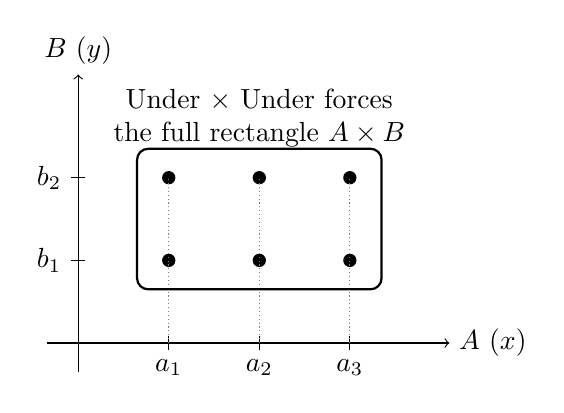
\begin{tikzpicture}[x=1.15cm,y=1.05cm]
  \draw[->] (-0.35,0) -- (4.1,0) node[right] {$A$ ($x$)};
  \draw[->] (0,-0.35) -- (0,3.25) node[above] {$B$ ($y$)};
  \foreach \x/\xl in {1/a_1,2/a_2,3/a_3} {
    \draw (\x,0.08)--(\x,-0.08) node[below] {$\xl$};
  }
  \foreach \y/\yl in {1/b_1,2/b_2} {
    \draw (0.08,\y)--(-0.08,\y) node[left] {$\yl$};
  }
  \foreach \x in {1,2,3} {
    \foreach \y in {1,2} {
      \fill (\x,\y) circle (2.4pt);
      \draw[densely dotted,gray] (\x,0)--(\x,\y);
    }
  }
  \draw[rounded corners,thick] (0.65,0.65) rectangle (3.35,2.35);
  \node[align=center] at (2,2.72) {Under $\times$ Under forces\\the full rectangle $A\times B$};
\end{tikzpicture}
\caption{For disjoint inhabited atomic Under formulas, every $A$-fiber covers
all of $B$, so fiber composition and separating product coincide.}
\label{fig:under-rectangle}
\end{figure}

For general formulas, the reverse implications fail.  The simplest failure
uses an Over atom.  Let
\[
  P\triangleq x:\{\Bool\mid\top\},
  \qquad
  Q\triangleq y:[\Bool\mid\top],
\]
and take the diagonal capability
\[
  r_{\mathrm{diag}}
  =\{(x=\false,y=\false),(x=\true,y=\true)\}.
\]
Then $r_{\mathrm{diag}}\modelsr Q\rfcomp P$: $Q$ covers both values of $y$,
and each fixed-$y$ fiber contains one safe Boolean $x$, which is enough for
the Over atom $P$.  However,
\[
  r_{\mathrm{diag}}\not\modelsr P*Q.
\]
The Under resource for $Q$ must contain both $y$ values, and its Cartesian
product with any nonempty Over witness for $P$ contains an off-diagonal point.
Thus $*$ is strictly stronger in general; Under is the exact fragment because
it forces the same complete canonical set in every fiber.

\section{Dependent type negation}

No new wand is needed: ordinary dependent arrows can repeatedly expose the
increasing fiber context.  Consider a function whose parameters and result
are all Over base types:
\begin{equation}\label{eq:safety-example}
  x:\{\mathsf{Nat}\mid\top\}\to
  y:\{\mathsf{Nat}\mid x<\nu\}\to
  \{\Bool\mid\psi(x,y,\nu)\}.
\end{equation}
A traditional negation changes each Over parameter into a disjoint Under
parameter and complements the result qualifier:
\begin{equation}\label{eq:old-negation}
  x:[\mathsf{Nat}\mid\top]\mathbin{-*}
  y:[\mathsf{Nat}\mid x<\nu]\mathbin{-*}
  [\Bool\mid\neg\psi(x,y,\nu)].
\end{equation}
The second separating premise is inappropriate: its resource must be
disjoint from $x$, while its qualifier simultaneously reads $x$.

Fiber refinement instead keeps ordinary arrows and accumulates all previously
visible variables in both later parameters and the final Under result:
\begin{equation}\label{eq:new-negation}
  x:[\mathsf{Nat}\mid\top]\to
  y:[\mathsf{Nat}\mid\{x\}.\{x<\nu\}]\to
  [\Bool\mid\{x,y\}.\{\neg\psi(x,y,\nu)\}].
\end{equation}
At formula level the parameter context is
\[
  (x:[\mathsf{Nat}\mid\top])
  \rfcomp
  (y:[\mathsf{Nat}\mid x<\nu]).
\]
For a further parameter $z$ depending on $x$ and $y$, the translation uses
\[
  z:[b\mid\{x,y\}.\{\psi(x,y,\nu)\}],
\]
or, equivalently, one more right-facing composition.  Negation therefore
changes every Over parameter into Under coverage and the final Over result
into the Under complement.  Dependencies remain expressible because each
successive type grows its fiber observation set instead of imposing
disjointness.

\section{Proof obligations}

A formal development should establish support-padding normalization, the two
entailments in~\eqref{eq:star-to-fiber}, and the atomic-Under characterization
\eqref{eq:under-equivalence}.  It should then formalize the Over diagonal
counterexample and prove that the fiber-accumulating translation
\eqref{eq:new-negation} correctly implements type negation for dependent
parameters.

\end{document}
